%! tex root = ../master.tex

\chapter{System Implementation}

\todo[inline, color=green]
{INTRO, to be reviewed}
This chapter deals with how the system\textquotesingle s functionalities 
are implemented. Diagrams will be included when necessary, as well as code 
snippets for the interesting parts of the program. In the end, all these
will be reviewed and compared with the actual requirements of the standard.


\section{Hardware}

\subsection{System clock}

\begin{figure}[H]
\centering
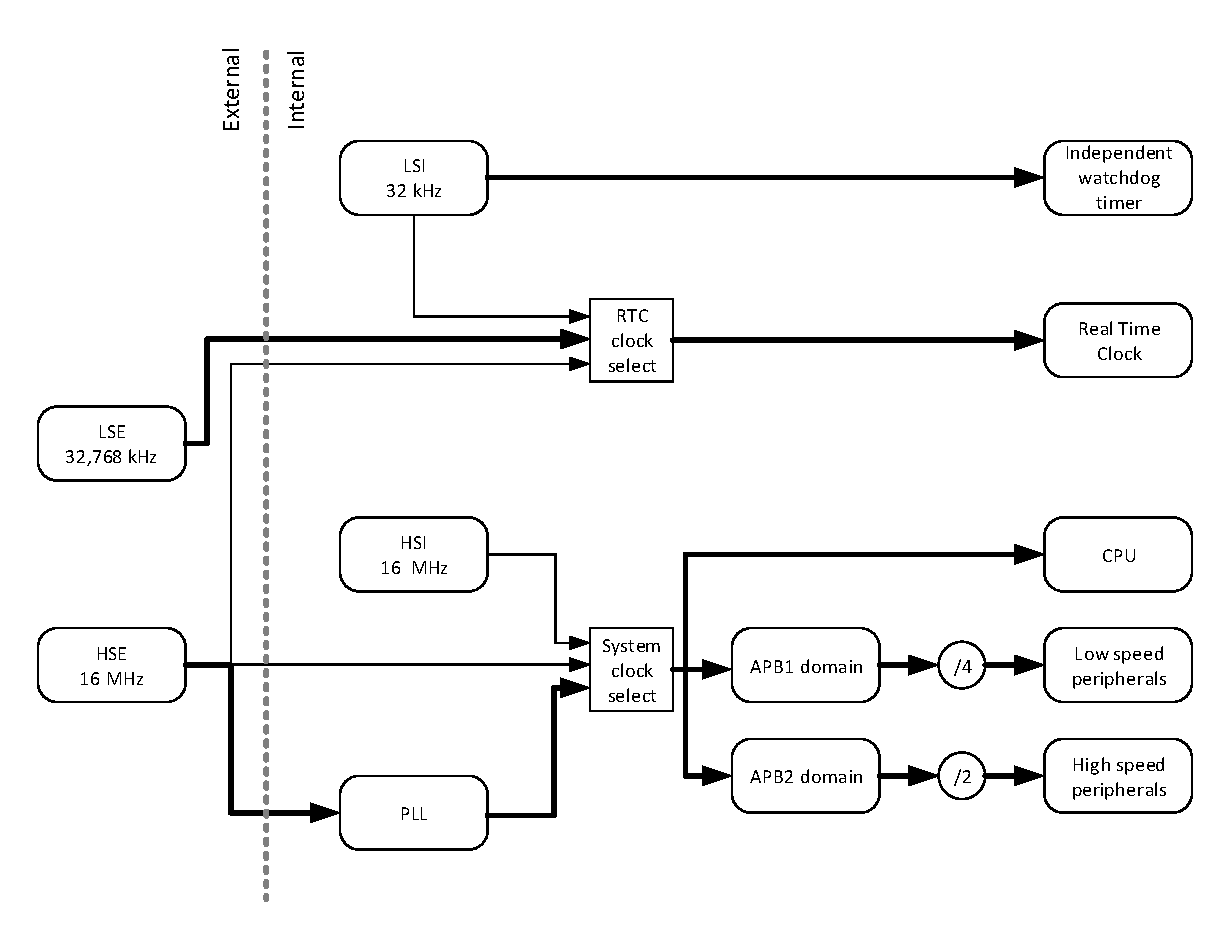
\includegraphics[width=\textwidth]{system_clock.pdf}
\captionof{figure}{An advanced system overview}
\label{fig:advanced_system}
\end{figure}

\section{Drivers}

\subsection{UART}

The UART sets the speed of the transmission and reception of the information between the STM32 and the outside. The communication is made by one character at a time. The transmission is activated by the interrupts and it can happen both ways simultaneously, or one way at a time. An UART has a clock generator, that we set for 16Mz, input and output registers, transmit/receive control, read/write control logic, and transmit/receiver buffers.
It is also possible to communicate with the UART using a screen, getting some important output for debugging.

\subsection{Watchdog timer}
% \ http://electronics.stackexchange.com/questions/123080/independent-watchdog-iwdg-or-window-watchdog-wwdg
The STM32 MCU has two watchdog timers ready to reset the program, in case of an error.
The first one, is the independent watchdog timer, based on an independent oscillator (32 kHz).
When initialised, the watchdog timer receives a value, from which it starts counting down, using
the ticks from the crystal. In the meanwhile, the program has to reset this count, by refreshing 
the timer to the same value it used before. If this fails to happen, when the count reaches zero, 
the watchdog timer will react by restarting the board.
\\
The second watchdog timer, is called a window watchdog. In contrast to the independent watchdog, 
one can provide a time interval in which the timer has to be reset. Resetting the timer outside this interval(as well as not resetting it in the mentioned time window) would restart the program. It uses 
the system clock, which means that if this fails, the watchdog won't be able to reset the system.

\subsubsection{Specifics}
The driver for the independent watchdog works by setting a prescaler on the 32kHz crystal to match 
the time requirements of the program(multiples of milliseconds). The watchdog is then initialised 
and started using the HAL library specific functions. \\
When the program is run, the watchdog restarts it after the interval of time set in the initialisation
phase runs out. In order to have the program running as usual, the refresh function has to be called,
 at intervals shorter than the initial time span.

\subsection{Timing function}
This driver is used for precise measuring the execution time of different functions. It uses the DWT
 registers defined in the ARM-M4 Architecture manual. These are responsible for Data Watchpoint 
 and Trace support. By using one of these counters, one could follow the system's clock ticks. 
 At a core frequency of 168 MHz, each tick would take 5.45 nanoseconds.\\
In order to do this, the DWT\textunderscore CONTROL register is set to a value that allows the system's clock to be sent to DWT\textunderscore CYCCNT. After this, the time can easily be tracked by converting the value of DWT\textunderscore CYCCNT.

\section{OS}

\subsection{Scheduler}

\subsubsection{Context Switching}
There are multiple different states the processor can be in, when the context switch from one process to another occurs.
The state determines whether the Master Stack Pointer or the Process Stack Pointer was used by the process,
and whether the FPU was used by the process or not. 
Because of this, the context switch algorithm must start by determining the processor state in order to know which registers
to save and where to save them to.\\
The processor state is saved in the Link return register, and it can be one of the possible six
EXC\_RETURN values (see figure \ref{tab:exc-return}).
The state is saved entirely on the stack. Therefore, it is important for the software to know which
stack pointer to use when saving the remaining registers.


\section{APEX}

\section{Partitions}

\section{Features of the system}
\todo[inline, color=green]{Here we can have a table showing what features
our system has, what features were not implemented, in regards to the
standard}
